\documentclass[conference]{IEEEtran}
\usepackage{amsmath,amssymb,amsfonts}
\usepackage{algorithmic}
\usepackage{graphicx}
\usepackage{textcomp}
\usepackage{xcolor}
\usepackage{booktabs}
\usepackage{multirow}
\usepackage{siunitx}
\usepackage{hyperref}
\usepackage{cite}
\usepackage{array}

\sisetup{per-mode=symbol}

\begin{document}

\pagestyle{plain}

\title{Reinforcement Learning for Thrust-Vectored Fin Control of an Electric Ducted Fan VTOL Vehicle in Simulation}

\author{
\IEEEauthorblockN{Tang Zijian (Jacob Tang)}
\IEEEauthorblockA{Department of Computer and Information Sciences \\
Minnesota State University, Mankato \\
Mankato, MN, USA}
}

\maketitle

\begin{abstract}
This paper presents a Proximal Policy Optimization (PPO) approach to attitude and position control of a thrust-vectored electric ducted fan (EDF) vertical take-off and landing (VTOL) vehicle using aerodynamic control fins immersed in the exhaust stream. Unlike conventional multirotor platforms that achieve control authority through differential rotor speeds, the vehicle studied here relies on a single axial EDF unit and four jet-vane fins for three-axis attitude control, presenting a tightly coupled, nonlinear control problem. We develop a GPU-accelerated simulation environment in NVIDIA Isaac Sim with semi-empirical aerodynamic, propulsion, and actuator dynamics models calibrated to a physical 3.1\,kg EDF drone testbed. A feed-forward actor--critic PPO agent with a 24-dimensional observation space and 5-dimensional continuous action space (four fin deflections plus throttle) is trained on 128 parallel environments for hover stabilization and autonomous landing tasks. The hover policy achieves a mean position error of \SI{0.085}{\metre} within 2{,}048 environment steps. The landing policy, trained over 5 million steps with spawn-position curriculum, achieves 100\% landing rate with a mean touchdown speed of \SI{0.126}{\metre\per\second}, though lateral accuracy (mean pad distance \SI{1.89}{\metre}) remains an open challenge. We detail the simulation architecture, reward design rationale, and training methodology, and discuss implications for sim-to-real transfer to the physical testbed.
\end{abstract}

\begin{IEEEkeywords}
reinforcement learning, thrust vector control, electric ducted fan, proximal policy optimization, VTOL, Isaac Sim, jet vane
\end{IEEEkeywords}

\section{Introduction}

Vertical take-off and landing (VTOL) vehicles have seen rapid adoption across commercial, military, and research domains. While conventional multirotors achieve attitude control through differential rotor speeds, alternative configurations---particularly those employing thrust vector control (TVC)---offer potential advantages in aerodynamic efficiency, noise reduction, and mechanical simplicity for certain mission profiles \cite{b1}.

Thrust-vectored vehicles that use aerodynamic control surfaces (jet vanes or fins) immersed in the exhaust stream of a single propulsion unit present a fundamentally different control challenge compared to multirotors. The control authority is coupled to the throttle state: at low thrust, fin effectiveness diminishes because the dynamic pressure in the exhaust drops quadratically with rotor speed. This throttle-dependent authority, combined with nonlinear aerodynamic force characteristics, actuator dynamics, and gyroscopic effects from the spinning rotor, makes classical linear control design challenging and motivates data-driven approaches.

Reinforcement learning (RL) has demonstrated success in quadrotor control \cite{b2, b3}, fixed-wing flight \cite{b4}, and rocket landing \cite{b5}. However, its application to thrust-vectored fin control of EDF vehicles remains largely unexplored. The key distinctions of this control problem include: (1) a single thrust source with four coupled control surfaces, (2) aerodynamic forces that depend on both fin deflection angle and instantaneous exhaust velocity, (3) significant actuator dynamics from hobby-grade servos, and (4) gyroscopic precession from the high-speed rotor.

This paper makes the following contributions:
\begin{itemize}
    \item A GPU-accelerated simulation environment for an EDF TVC drone built on NVIDIA Isaac Sim with physically grounded aerodynamic, propulsion, and actuator models.
    \item A PPO-based control policy for hover stabilization and autonomous landing of a thrust-vectored vehicle, trained end-to-end from raw state observations.
    \item Analysis of reward design considerations specific to TVC vehicles, including the terminal-vs-per-step magnitude balance critical for landing tasks.
    \item Preliminary training results demonstrating feasibility and identifying open challenges for lateral accuracy in landing.
\end{itemize}


\section{Related Work}

\subsection{Reinforcement Learning for Aerial Vehicle Control}

RL-based control of aerial vehicles has progressed significantly in recent years. Hwangbo et al.\ demonstrated that PPO could learn agile quadrotor control policies that transfer to hardware \cite{b2}. Koch et al.\ applied deep RL to quadrotor attitude control, comparing multiple algorithms and finding that PPO provided robust training stability \cite{b3}. Pi et al.\ showed that RL policies trained in simulation could achieve robust quadrotor flight under wind disturbances after sim-to-real transfer \cite{b4}.

GPU-accelerated parallel simulation has been a key enabler. Rudin et al.\ demonstrated that massively parallel environments in Isaac Gym could train locomotion policies orders of magnitude faster than prior approaches \cite{b6}. Makoviychuk et al.\ extended this to manipulation tasks with thousands of parallel environments \cite{b7}.

\subsection{Transformer-Based Memory for Long-Horizon Control}

Landing tasks are inherently long-horizon: the controller must plan a descent trajectory over hundreds of decision steps while inferring slowly varying disturbances from local state snapshots. Standard feed-forward policies lack temporal context beyond the current observation. Transformer-XL \cite{b17} addresses this through segment-level recurrence, and Gated Transformer-XL (GTrXL) \cite{b16} stabilizes transformer training in RL by gating the residual connections. Li et al.\ \cite{b18} survey the use of transformers in RL and argue that they are most beneficial when long-range temporal credit assignment matters more than raw simplicity.

In aerospace guidance, Federici et al.\ \cite{b19} applied meta-reinforcement learning with transformers to lunar landing, and Carradori et al.\ \cite{b20} demonstrated transformer-based robust feedback guidance for atmospheric powered landing. Both studies report strong simulated performance under uncertain initial conditions and disturbances, but neither closes the loop on hardware transfer---a gap that motivates the physical testbed described in this work.

\subsection{Thrust Vector Control}

TVC has a long history in rocketry, where gimbaled nozzles or jet vanes provide attitude control during powered flight \cite{b8}. More recently, TVC has been explored for VTOL vehicles. Jet-vane TVC, where flat plates are immersed in the exhaust stream, provides a mechanically simple alternative to gimbaled motors but introduces nonlinear aerodynamic coupling \cite{b9}.

Classical control approaches for TVC vehicles typically linearize the plant around a hover operating point and apply PID or LQR controllers \cite{b10}. However, the strongly nonlinear relationship between fin deflection, throttle state, and resulting forces---particularly the quadratic dependence of fin effectiveness on exhaust velocity---limits the operating envelope of linear controllers. Optimization-based guidance such as Sequential Convex Programming (SCP) offers fuel-aware trajectory planning \cite{b21}, but trust-region limitations can cause infeasibility when the required maneuver deviates significantly from the nominal trajectory.

\subsection{Sim-to-Real Transfer}

Domain randomization \cite{b11} and system identification \cite{b12} are established techniques for bridging the simulation-to-reality gap. For aerial vehicles, Sadeghi and Levine demonstrated that policies trained entirely in simulation could transfer to real quadrotors \cite{b13}. The fidelity of the simulation dynamics model is a critical factor, motivating the semi-empirical approach adopted in this work.

\section{Vehicle Description}

\subsection{Physical Platform}

The testbed is a custom-built EDF VTOL vehicle (Fig.~\ref{fig:drone_schematic}) with the following specifications:

\begin{figure}[htbp]
\centering
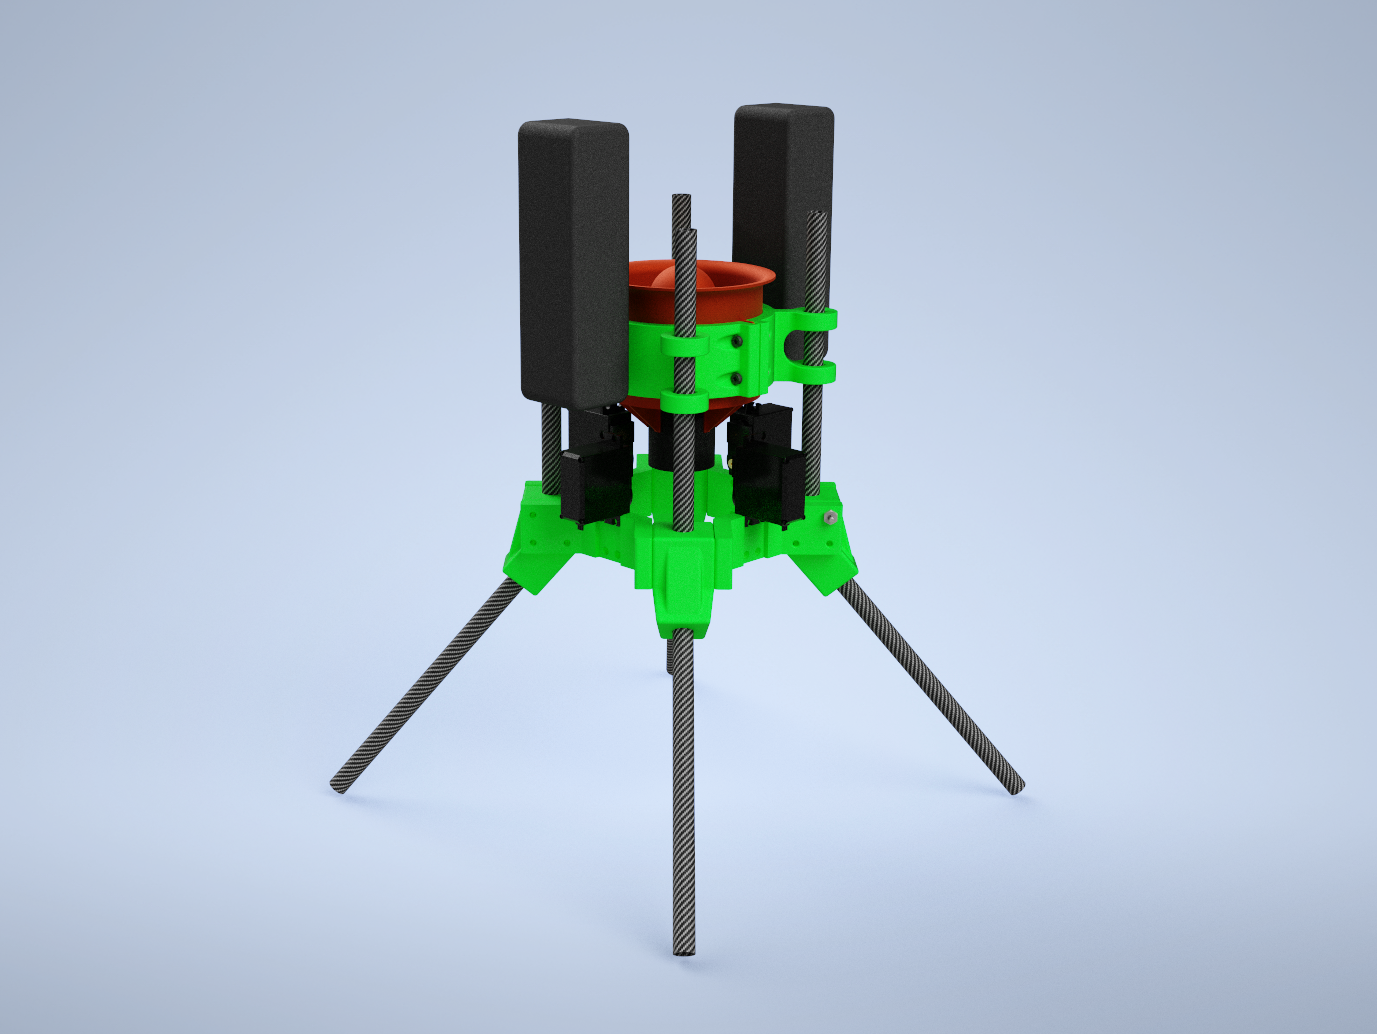
\includegraphics[width=0.75\columnwidth]{figures/cad_v1.png}
\caption{CAD rendering of the EDF TVC drone testbed showing the single axial EDF unit, four cruciform jet-vane fins, MG996R servo actuators, carbon-fiber frame, battery, and landing legs.\protect\footnotemark}
\label{fig:drone_schematic}
\end{figure}
\footnotetext{Not all structural components are shown; only the core EDF unit, servos, frame, battery, and legs are present in this rendering.}

\begin{table}[htbp]
\caption{Vehicle Physical Parameters}
\label{tab:vehicle_params}
\centering
\begin{tabular}{lrl}
\toprule
\textbf{Parameter} & \textbf{Value} & \textbf{Source} \\
\midrule
Total mass & \SI{3.1}{\kilogram} & Measured \\
Body length & \SI{0.35}{\metre} & Measured \\
Body diameter & \SI{0.12}{\metre} & Measured \\
$I_{xx}$, $I_{yy}$ & \SI{0.05}{\kilogram\metre\squared} & Isaac Sim MassAPI \\
$I_{zz}$ & \SI{0.02}{\kilogram\metre\squared} & Isaac Sim MassAPI \\
Fin count & 4 & --- \\
Fin area (each) & \SI{0.002}{\metre\squared} & Measured \\
Max fin deflection & \SI{15}{\degree} (\SI{0.262}{\radian}) & Measured \\
\bottomrule
\end{tabular}
\end{table}

The vehicle employs a single FMS 90\,mm 12-blade EDF unit (FMSDF010-1) with a 4068-KV1850 inrunner motor powered by a 6S LiPo battery. Four MG996R hobby servos actuate flat-plate jet vanes positioned in the EDF exhaust stream. The fins are arranged in a cruciform pattern at $90°$ intervals, with hinge axes oriented to provide independent pitch, roll, and yaw authority through differential deflection.

\subsection{Control Architecture}

The vehicle's control surfaces are arranged as follows:
\begin{itemize}
    \item \textbf{Forward fin} (+X): hinge axis along +Y, provides pitch control.
    \item \textbf{Right fin} (+Y): hinge axis along $-$X, provides roll control.
    \item \textbf{Aft fin} ($-$X): hinge axis along $-$Y, complementary pitch.
    \item \textbf{Left fin} ($-$Y): hinge axis along +X, complementary roll.
\end{itemize}

Yaw control is achieved through differential deflection that creates asymmetric tangential forces. Altitude is controlled via the EDF throttle. This architecture provides full 6-DOF control authority (three rotational axes plus altitude) through five actuator commands: four fin angles and one throttle.


\section{Simulation Environment}

\subsection{Coordinate Frames}

The simulation uses two coordinate conventions. The Isaac Sim world frame is right-handed and Z-up ($+x$ forward, $+y$ left, $+z$ up). Internal control and aerodynamic calculations use a body-fixed forward-right-down (FRD) frame ($+x$ forward, $+y$ right, $+z$ down). A single conversion boundary between these frames is enforced through:

\begin{equation}
\mathbf{R}_{I\leftarrow F} =
\begin{bmatrix}
1 & 0 & 0 \\
0 & -1 & 0 \\
0 & 0 & -1
\end{bmatrix}
\label{eq:frd_isaac_map}
\end{equation}

\noindent A body-FRD vector is mapped to world coordinates by $\mathbf{v}^{W} = \mathbf{R}(\mathbf{q})\,\mathbf{R}_{I\leftarrow F}\,\mathbf{v}^{F}$, where $\mathbf{R}(\mathbf{q})$ is the rotation matrix induced by the vehicle quaternion $\mathbf{q} = [w,x,y,z]^T$. Vehicle orientation uses the quaternion representation throughout to avoid gimbal lock.

\subsection{Overview}

The simulation environment is built on NVIDIA Isaac Sim using the Isaac Lab framework (v2.3.2), which provides GPU-accelerated rigid-body physics via PhysX 5. The environment implements a Gymnasium-compatible interface with vectorized step, reset, and observation computation across 128 parallel environments on a single GPU.

The simulation operates at a physics timestep of $\Delta t_{\text{phys}} = \SI{8.33}{\milli\second}$ ($\SI{120}{\hertz}$) with a decimation factor of 4, yielding an RL decision timestep of $\Delta t_{\text{RL}} = \SI{33.3}{\milli\second}$ ($\SI{30}{\hertz}$). Each RL step executes four physics substeps, during which actuator dynamics, aerodynamic forces, and propulsion effects are updated at the full physics rate.

\begin{figure}[htbp]
\centering
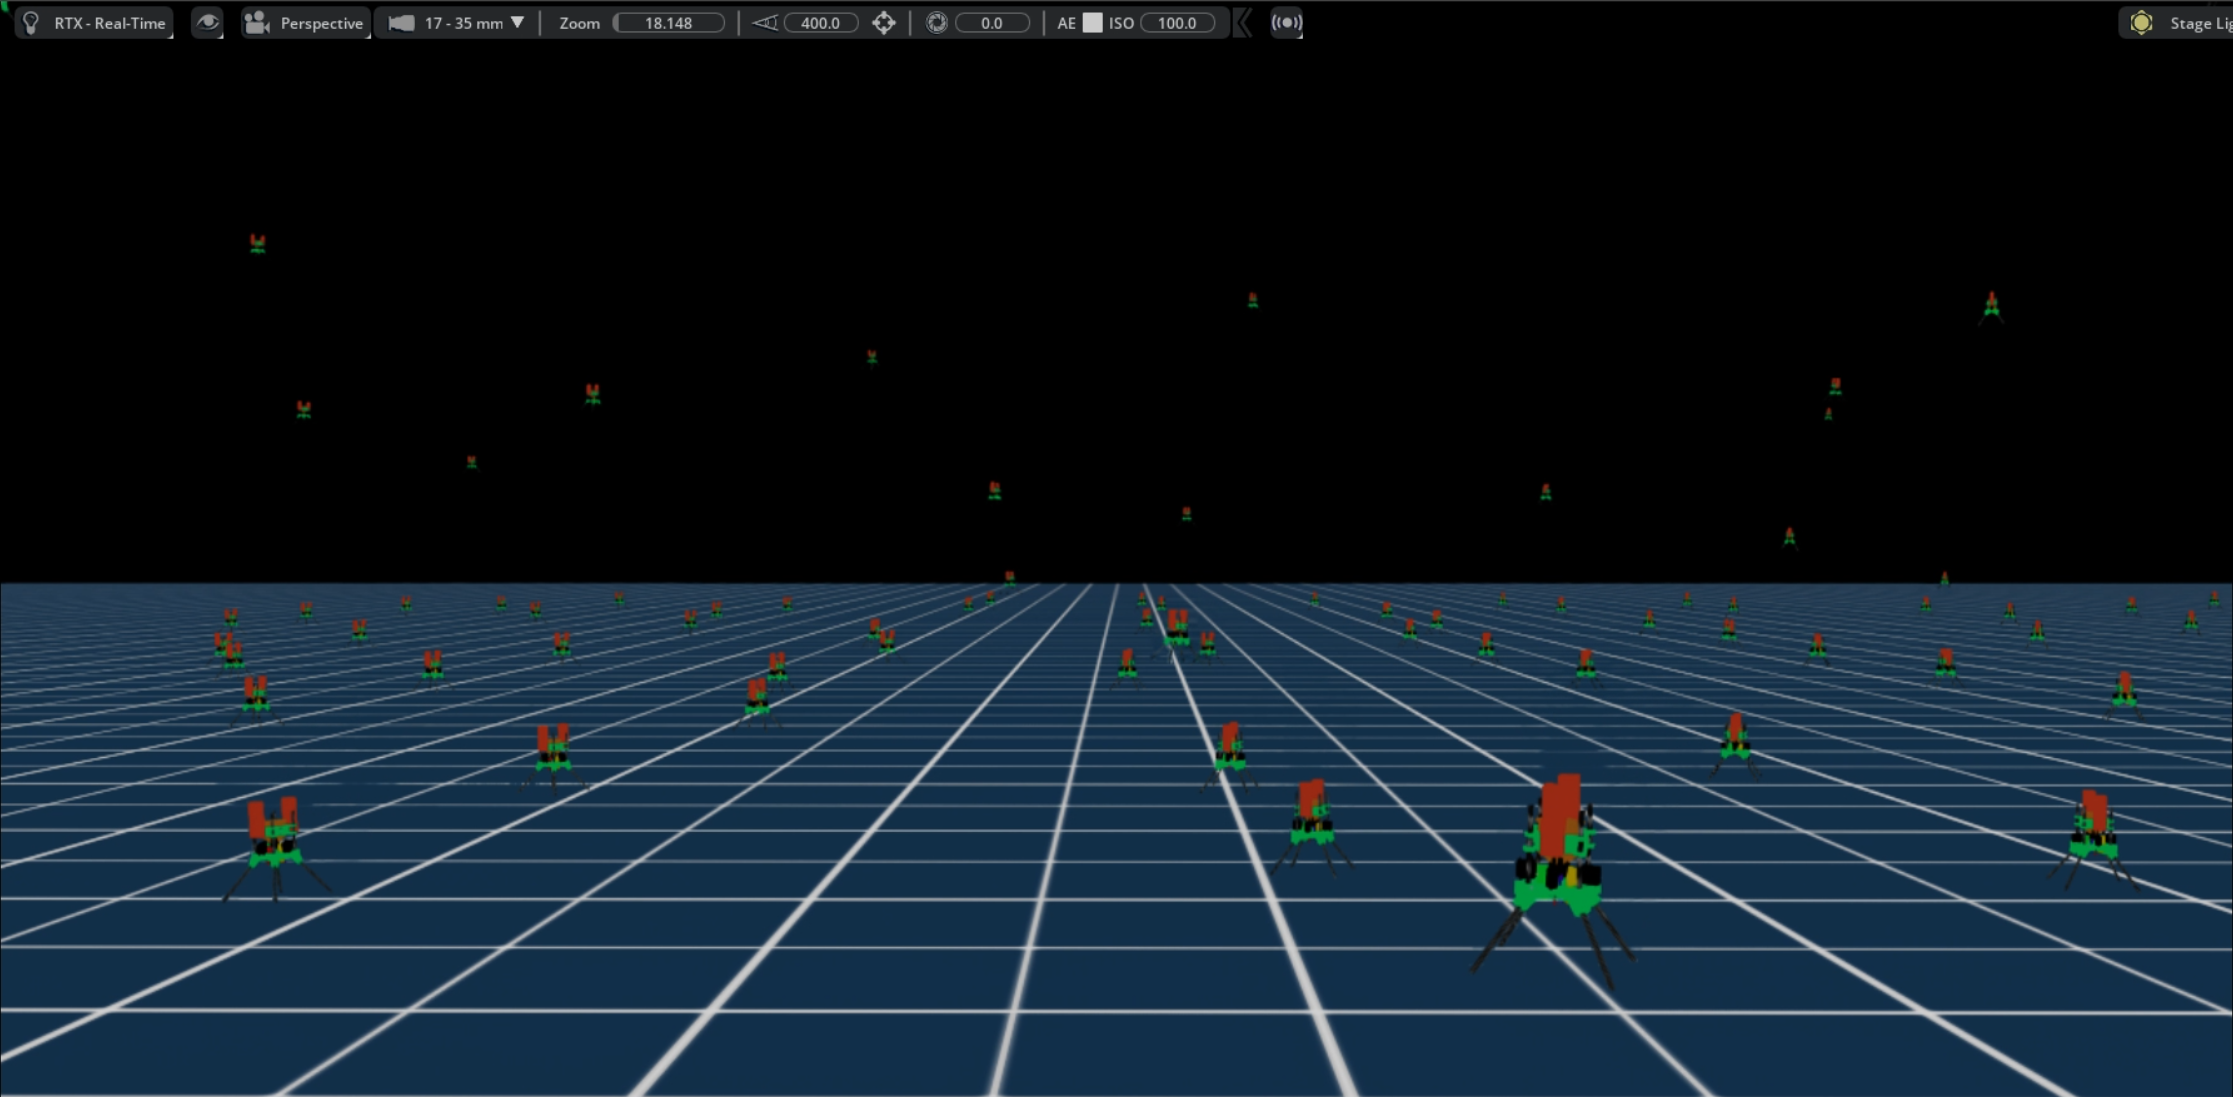
\includegraphics[width=\columnwidth]{figures/isaacsim_128_env.png}
\caption{NVIDIA Isaac Sim viewport showing 128 parallel EDF drone instances during a headed training run. Each vehicle is spawned at a randomized position and orientation within the configured spawn box and executes the landing task simultaneously on the GPU.}
\label{fig:isaac_sim_envs}
\end{figure}

\subsection{Propulsion Model}

The EDF propulsion system is modeled with first-order spool dynamics and a quadratic thrust law:

\begin{equation}
\dot{\omega} = \frac{\omega_{\text{target}} - \omega}{\tau_{\text{motor}}}
\label{eq:spool}
\end{equation}

\begin{equation}
T = k_T \omega^2
\label{eq:thrust}
\end{equation}

\noindent where $\omega$ is the rotor angular velocity, $\omega_{\text{target}} = u_{\text{throttle}} \cdot \omega_{\max}$ is the commanded speed, $\tau_{\text{motor}} = \SI{0.15}{\second}$ is the motor time constant, and $k_T = T_{\max} / \omega_{\max}^2$ is the thrust coefficient derived from the maximum thrust $T_{\max} = \SI{39.2}{\newton}$ and maximum angular velocity $\omega_{\max} = \SI{4300}{\radian\per\second}$.

The propulsion model also computes three torque components acting on the vehicle body:

\begin{enumerate}
    \item \textbf{Static reaction torque}: $\boldsymbol{\tau}_{\text{static}} = -k_Q \omega^2 \hat{\mathbf{e}}_z$, opposing the rotor spin direction.
    \item \textbf{Dynamic spool torque}: $\boldsymbol{\tau}_{\text{spool}} = -I_{\text{rotor}} \dot{\omega} \hat{\mathbf{e}}_z$, the reaction to rotor acceleration.
    \item \textbf{Gyroscopic precession}: $\boldsymbol{\tau}_{\text{gyro}} = -\boldsymbol{\omega}_{\text{body}} \times (I_{\text{rotor}} \omega \hat{\mathbf{e}}_z)$, coupling body rotation to rotor angular momentum.
\end{enumerate}

\begin{table}[htbp]
\caption{EDF Propulsion Parameters}
\label{tab:edf_params}
\centering
\begin{tabular}{lrl}
\toprule
\textbf{Parameter} & \textbf{Value} & \textbf{Source} \\
\midrule
Max thrust $T_{\max}$ & \SI{39.2}{\newton} & Datasheet \\
Motor time constant $\tau_{\text{motor}}$ & \SI{0.15}{\second} & Estimate \\
Max angular velocity $\omega_{\max}$ & \SI{4300}{\radian\per\second} & Derived \\
Rotor inertia $I_{\text{rotor}}$ & \SI{0.0002}{\kilogram\metre\squared} & Estimate \\
Exhaust speed (nominal) & \SI{116}{\metre\per\second} & Estimate \\
Gyro torque scale & 0.1 & Calibrated \\
\bottomrule
\end{tabular}
\end{table}

\subsection{Fin Aerodynamic Model}

The jet-vane aerodynamic forces are computed using a semi-empirical model. Each fin experiences a dynamic pressure proportional to the square of the exhaust velocity, which itself scales with throttle:

\begin{equation}
q = \frac{1}{2} \rho \, v_{\text{exhaust}}^2 \cdot u_{\text{throttle}}^2 \cdot k_{\text{duct}}
\label{eq:dynamic_pressure}
\end{equation}

\noindent where $\rho = \SI{1.225}{\kilogram\per\metre\cubed}$ is air density, $v_{\text{exhaust}} = \SI{116}{\metre\per\second}$ is the nominal exhaust speed, $u_{\text{throttle}} \in [0, 1]$ is the normalized throttle, and $k_{\text{duct}} = 1.3$ is a duct confinement correction factor.

The normal (lift) and tangential (drag) force coefficients are:

\begin{equation}
C_N(\alpha) = C_{N_\alpha} \cdot \alpha \cdot (1 - k_{\text{sat}} \alpha^2)
\label{eq:cn}
\end{equation}

\begin{equation}
C_D(\alpha) = C_{D_0} + C_{D_{\alpha^2}} \alpha^2
\label{eq:cd}
\end{equation}

\noindent where $\alpha$ is the fin deflection angle, $C_{N_\alpha} = 3.5\,\text{rad}^{-1}$ is the lift-curve slope (derived from thin-airfoil theory with empirical correction), $k_{\text{sat}} = 2.0$ accounts for stall saturation, $C_{D_0} = 0.05$ is the zero-deflection drag, and $C_{D_{\alpha^2}} = 1.5$ captures the deflection-dependent drag increase.

The resulting forces per fin are:
\begin{equation}
F_n = q \cdot S_{\text{fin}} \cdot C_N(\alpha), \quad F_t = q \cdot S_{\text{fin}} \cdot C_D(\alpha)
\label{eq:fin_forces}
\end{equation}

\noindent where $S_{\text{fin}} = \SI{0.002}{\metre\squared}$. The normal force $F_n$ acts perpendicular to the exhaust flow (providing lateral control force), while the tangential force $F_t$ opposes the flow (contributing to thrust loss). The total thrust loss from all four fins is subtracted from the EDF thrust before application.

A critical feature of this model is the quadratic coupling between throttle and fin effectiveness: at 50\% throttle, fin forces are only 25\% of their maximum value. This coupling is a defining characteristic of jet-vane TVC and distinguishes it from conventional multirotor control.

\subsection{Force Application}

The simulation supports two force dispatch modes. In the default \emph{per-link force} mode, each fin force is rotated to world coordinates and applied at its world-frame center-of-pressure location using Isaac Lab's wrench composer, while EDF thrust and wind drag are applied as body-link forces. This allows the articulation physics engine to generate the resulting vehicle torques from geometry rather than from manually synthesized body moments. An optional \emph{collapsed body wrench} mode forms a net body force and geometric torque $\boldsymbol{\tau}^{F}_{\text{fin}} = \sum_{i=1}^{4}\mathbf{r}_i^{F}\times \mathbf{F}_{i}^{F}$ before applying a single body wrench, which is useful for debugging and validation.

\subsection{Servo Actuator Model}

The MG996R servo dynamics are modeled as a first-order lag with rate limiting and deadband:

\begin{equation}
\dot{\alpha}_{\text{fin}} = \text{clip}\!\left(\frac{\alpha_{\text{cmd}} - \alpha_{\text{fin}}}{\tau_{\text{servo}}},\; -\dot{\alpha}_{\max},\; \dot{\alpha}_{\max}\right)
\label{eq:servo}
\end{equation}

\noindent where $\tau_{\text{servo}} = \SI{0.05}{\second}$, $\dot{\alpha}_{\max} = \SI{7.54}{\radian\per\second}$ (derived from the datasheet $60°$ transit time of \SI{0.14}{\second}), and a deadband of \SI{0.017}{\radian} ($\approx 1°$) suppresses response to commands smaller than the mechanical resolution. The servo state is clamped to $\pm\SI{0.262}{\radian}$ ($\pm 15°$).

\subsection{Contact Detection and State Machine}

Landing and crash detection use a four-state contact state machine:

\begin{enumerate}
    \item \textbf{AIRBORNE}: No ground contact detected.
    \item \textbf{GROUND\_CONTACT\_CANDIDATE}: Contact detected; dwell counter incrementing.
    \item \textbf{LANDED}: Dwell counter exceeds threshold (15 consecutive frames at \SI{120}{\hertz} $= \SI{0.125}{\second}$).
    \item \textbf{CRASHED}: Crash criteria met (excessive tilt, angular rate, or impact speed).
\end{enumerate}

Contact is detected via a kinematic proxy: height $< \SI{0.40}{\metre}$ and downward velocity $< \SI{0.50}{\metre\per\second}$. The dwell requirement prevents transient bounces from registering as landings.

\subsection{Wind and Drag Model}

Aerodynamic body drag is modeled as:
\begin{equation}
\mathbf{F}_{\text{drag}} = -\frac{1}{2} \rho \, C_d \, A_{\text{ref}} \, |\mathbf{v}_{\text{rel}}|^2 \, \hat{\mathbf{v}}_{\text{rel}}
\label{eq:drag}
\end{equation}

\noindent where $C_d = 1.0$ (bluff body estimate), $A_{\text{ref}} = \SI{0.02}{\metre\squared}$, and $\mathbf{v}_{\text{rel}}$ is the body velocity relative to the wind field. The wind model supports steady-state wind vectors and stochastic gust events with configurable magnitude, duration, and interval, though the results presented here use nominal (zero-wind) conditions.


\section{Learning Algorithm}

\subsection{Proximal Policy Optimization}

We employ Proximal Policy Optimization (PPO) \cite{b14} with clipped surrogate objectives. PPO is an on-policy actor--critic algorithm that constrains policy updates to a trust region, preventing destructively large gradient steps while maintaining sample efficiency. The clipped objective is:

\begin{equation}
L^{\text{CLIP}}(\theta) = \hat{\mathbb{E}}_t \left[ \min\!\left( r_t(\theta) \hat{A}_t,\; \text{clip}(r_t(\theta), 1{-}\epsilon, 1{+}\epsilon) \hat{A}_t \right) \right]
\label{eq:ppo_clip}
\end{equation}

\noindent where $r_t(\theta) = \pi_\theta(a_t | s_t) / \pi_{\theta_{\text{old}}}(a_t | s_t)$ is the probability ratio, $\hat{A}_t$ is the Generalized Advantage Estimate (GAE) \cite{b15}, and $\epsilon = 0.2$ is the clipping coefficient. An adaptive KL-divergence early stopping criterion ($\text{KL}_{\text{target}} = 0.03$) provides an additional safeguard against policy collapse.

Advantages are computed using GAE with $\lambda = 0.95$ and discount factor $\gamma = 0.99$:

\begin{equation}
\hat{A}_t = \sum_{l=0}^{T-t} (\gamma \lambda)^l \delta_{t+l}, \quad \delta_t = r_t + \gamma V(s_{t+1}) - V(s_t)
\label{eq:gae}
\end{equation}

The combined loss function optimized at each update is:

\begin{equation}
L(\theta) = L^{\text{CLIP}}(\theta) - c_1 L^{\text{VF}}(\theta) + c_2 H[\pi_\theta]
\label{eq:total_loss}
\end{equation}

\noindent where $L^{\text{VF}}$ is the value function mean-squared error loss ($c_1 = 0.5$), and $H[\pi_\theta]$ is the policy entropy bonus ($c_2 = 0.005$) that encourages exploration.

\subsection{Observation Space}

The agent receives a 24-dimensional observation vector at each decision step:

\begin{table}[htbp]
\caption{Observation Space}
\label{tab:obs_space}
\centering
\begin{tabular}{clc}
\toprule
\textbf{Index} & \textbf{Component} & \textbf{Dim} \\
\midrule
0--2 & Position error (m) & 3 \\
3--6 & Attitude quaternion $[w,x,y,z]$ & 4 \\
7--9 & Linear velocity, body FRD (m/s) & 3 \\
10--12 & Angular velocity, body FRD (rad/s) & 3 \\
13 & Height above ground (m) & 1 \\
14--17 & Fin angles (rad) & 4 \\
18--21 & Fin angular rates (rad/s) & 4 \\
22 & Motor RPM, normalized $[0,1]$ & 1 \\
23 & Contact state (int $\to$ float) & 1 \\
\bottomrule
\end{tabular}
\end{table}

Position error is computed as the vector from the current position to the task target (hover setpoint or landing pad center). The quaternion representation avoids gimbal lock singularities inherent in Euler angles. Fin angles and rates provide proprioceptive feedback on actuator state, which is critical given the first-order servo lag. The normalized motor RPM informs the policy of available fin authority, since fin effectiveness scales quadratically with rotor speed.

\subsection{Action Space}

The action space is a 5-dimensional continuous vector:

\begin{equation}
\mathbf{a} = [\alpha_1, \alpha_2, \alpha_3, \alpha_4, u_{\text{throttle}}]
\label{eq:action}
\end{equation}

\noindent where $\alpha_i \in [-0.262, +0.262]$\,rad ($\pm 15°$) are the four fin deflection commands and $u_{\text{throttle}} \in [0, 1]$ is the normalized throttle. The network outputs are in $(-1, 1)$ via $\tanh$ saturation; fin channels are linearly scaled to $\pm 0.262$\,rad and the throttle channel is mapped via $(z + 1)/2$.

\subsection{Network Architecture}

Both the actor (policy) and critic (value function) are implemented as separate two-layer fully connected networks with 256 hidden units per layer and $\tanh$ activations (Fig.~\ref{fig:network_arch}). The actor outputs 5 action means; the exploration noise is parameterized by a learnable per-dimension log-standard-deviation vector. The critic outputs a single scalar state value.

\begin{figure}[htbp]
\centering
\fbox{\parbox{0.9\columnwidth}{\centering\vspace{1.5em}
\textbf{Actor Network}\\[0.5em]
Obs (24) $\to$ FC(256) $\to$ Tanh $\to$ FC(256) $\to$ Tanh $\to$ FC(5)\\[1em]
\textbf{Critic Network}\\[0.5em]
Obs (24) $\to$ FC(256) $\to$ Tanh $\to$ FC(256) $\to$ Tanh $\to$ FC(1)
\vspace{1.5em}}}
\caption{Actor--critic network architecture. Both networks take the 24-dimensional observation as input. The actor produces 5 action means; per-dimension log-standard-deviations are learned as free parameters.}
\label{fig:network_arch}
\end{figure}

Two initialization choices are critical for stable early training:

\begin{enumerate}
    \item \textbf{Throttle bias initialization.} The actor output layer bias for the throttle channel is initialized to $\text{atanh}(2 \cdot 0.78 - 1) \approx 1.05$, so the initial mean throttle maps to $\approx 0.78$---slightly below the hover throttle of $\sqrt{mg / T_{\max}} \approx 0.88$. This ensures initial rollouts straddle the productive hover/descent basin rather than free-falling from the default $0.5$ throttle.
    \item \textbf{Per-channel exploration noise.} Fin channels are initialized with $\log\sigma = -2.0$ (std $\approx 0.14$), while the throttle channel uses $\log\sigma = -1.0$ (std $\approx 0.37$). This asymmetry prevents excessive lateral noise from the fins while maintaining sufficient throttle exploration for altitude control.
\end{enumerate}

\subsection{Training Procedure}

Training uses 128 parallel environments on a single NVIDIA GPU. Each PPO update collects a rollout of 128 steps per environment (16{,}384 transitions total), then performs 4 epochs of minibatch gradient descent with 8 minibatches per epoch. The optimizer is Adam with learning rate $3 \times 10^{-4}$ and gradient norm clipping at 0.5.

\begin{table}[htbp]
\caption{PPO Hyperparameters (Landing Task)}
\label{tab:ppo_params}
\centering
\begin{tabular}{lr}
\toprule
\textbf{Parameter} & \textbf{Value} \\
\midrule
Parallel environments & 128 \\
Rollout length & 128 steps \\
Minibatches per update & 8 \\
Update epochs & 4 \\
Learning rate & $3 \times 10^{-4}$ \\
Discount $\gamma$ & 0.99 \\
GAE $\lambda$ & 0.95 \\
Clip coefficient $\epsilon$ & 0.2 \\
Entropy coefficient & 0.005 \\
Value loss coefficient & 0.5 \\
Max gradient norm & 0.5 \\
Target KL & 0.03 \\
\bottomrule
\end{tabular}
\end{table}

For the hover task, training runs for 2{,}048 environment steps with a residual-PID architecture: a PID baseline controller provides the nominal action, and the PPO policy learns a bounded residual correction scaled by 0.05. The hover task uses a smaller rollout length (64 steps), 2 minibatches, 2 update epochs, and a reduced learning rate ($10^{-6}$) to avoid destabilizing the PID baseline. For the landing task, training runs for 5{,}000{,}000 environment steps with pure PPO (no PID baseline), as the landing maneuver requires the policy to learn the full descent-to-touchdown trajectory.

\subsection{Spawn-Position Curriculum}

The landing task employs a linear spawn-position curriculum to address the exploration challenge of learning precision landing from large initial offsets. Training begins with a narrow spawn box of $\pm 0.5$\,m in the horizontal plane (XY), which linearly anneals to the full $\pm 2.0$\,m evaluation range over the first 3{,}000{,}000 steps. The altitude spawn range ($8$--$12$\,m) remains constant throughout. This curriculum allows the policy to first learn on-pad touchdown behavior before generalizing to larger lateral offsets.

Evaluation is always conducted against the full (un-curricularized) spawn range to ensure reported metrics reflect the final task difficulty.


\section{Reward Design}

Reward shaping is a critical design decision for TVC landing, where the agent must simultaneously manage altitude, lateral position, attitude, and touchdown conditions. We structure the reward as a sum of weighted per-step shaping terms and one-time terminal events.

\subsection{Per-Step Shaping Terms}

The per-step reward at each decision step is:

\begin{equation}
r_{\text{step}} = \sum_{i} w_i \cdot \phi_i(s_t, a_t)
\label{eq:step_reward}
\end{equation}

\noindent where $\phi_i$ are individual reward terms and $w_i$ are their weights. Table~\ref{tab:reward_weights} lists all terms and their weights for the landing task.

\begin{table}[htbp]
\caption{Landing Task Reward Weights}
\label{tab:reward_weights}
\centering
\begin{tabular}{lr}
\toprule
\textbf{Term} & \textbf{Weight} \\
\midrule
\multicolumn{2}{l}{\textit{Per-step shaping}} \\
Alive bonus & $+0.10$ \\
3D position error & $-0.05$ \\
Horizontal position error & $-0.30$ \\
Attitude error (tilt) & $-0.20$ \\
Angular velocity & $-0.10$ \\
Control effort (fin $|\alpha|$) & $-0.02$ \\
Control rate (fin $|\dot{\alpha}|$) & $-0.01$ \\
Vertical speed shaping & $-0.30$ \\
Delta-v cost $(T/T_{\max})^2$ & $-0.20$ \\
\midrule
\multicolumn{2}{l}{\textit{Terminal events}} \\
Crash penalty & $-200$ \\
Touchdown softness & $+25 \cdot e^{-v_{\text{impact}}}$ \\
Pad accuracy & $+200 \cdot e^{-d_{\text{horiz}}}$ \\
Landing success & $+250$ \\
\bottomrule
\end{tabular}
\end{table}

\subsection{Terminal-vs-Per-Step Magnitude Balance}

A key insight for landing reward design is the magnitude balance between integrated per-step costs and one-time terminal rewards. For an episode of length $T$ steps, the integrated per-step contribution is $\sum_i |w_i| \cdot \bar{\phi}_i \cdot T$, which can easily reach $\mathcal{O}(100)$ over a 30-second episode at 30\,Hz ($T = 900$). If terminal rewards are not substantially larger, PPO will optimize per-step cost minimization---typically by reducing throttle to zero---rather than pursuing the terminal landing event.

We set terminal magnitudes ($|w_{\text{terminal}}| \geq 200$) to clearly dominate the integrated per-step budget. The landing success bonus of $+250$ plus the pad accuracy bonus (up to $+200$) provide a combined terminal reward of up to $+450$ for a perfect landing, which exceeds the worst-case integrated per-step cost. The crash penalty of $-200$ ensures that uncontrolled impacts are strongly discouraged.

\subsection{Horizontal Guidance Shaping}

The horizontal position error term ($w = -0.30$) provides a dense gradient toward the landing pad throughout the descent. This term is independent of altitude, so the agent receives lateral guidance even at high altitudes where the pad accuracy terminal bonus (which uses $e^{-d_{\text{horiz}}}$) has negligible gradient. The vertical speed shaping term ($w = -0.30$) penalizes deviation from a target descent rate of approximately $0.5$\,m/s, encouraging a controlled descent profile rather than a ballistic drop.


\section{Experimental Results}

We present results for two tasks: hover stabilization and autonomous landing. All experiments use nominal (zero-wind) conditions. Evaluation metrics are computed over 128 parallel episodes with the full (un-curricularized) spawn range.

\subsection{Hover Stabilization}

The hover policy uses a residual-PID architecture where a PID controller provides the baseline action and the PPO policy learns a small bounded correction (scale $= 0.05$). After 2{,}048 environment steps of training, the policy achieves:

\begin{table}[htbp]
\caption{Hover Stabilization Results}
\label{tab:hover_results}
\centering
\begin{tabular}{lr}
\toprule
\textbf{Metric} & \textbf{Value} \\
\midrule
Mean position error & \SI{0.085}{\metre} \\
Max position error & \SI{0.215}{\metre} \\
Mean tilt & \SI{< 0.001}{\radian} \\
Max tilt & \SI{< 0.001}{\radian} \\
Mean angular rate & \SI{1.1e-5}{\radian\per\second} \\
Evaluation passed & Yes \\
\bottomrule
\end{tabular}
\end{table}

The near-zero tilt and angular rate values indicate that the PID baseline provides effective attitude stabilization, while the RL residual corrects for position drift. The mean position error of \SI{0.085}{\metre} is well within the \SI{0.5}{\metre} success threshold.

\subsection{Autonomous Landing}

The landing policy is trained with pure PPO (no PID baseline) for 5{,}000{,}000 environment steps with spawn-position curriculum. Table~\ref{tab:landing_results} summarizes the final evaluation metrics.

\begin{table}[htbp]
\caption{Landing Task Final Evaluation Results}
\label{tab:landing_results}
\centering
\begin{tabular}{lr}
\toprule
\textbf{Metric} & \textbf{Value} \\
\midrule
Landing rate & 100\% \\
Mean touchdown speed & \SI{0.126}{\metre\per\second} \\
Max touchdown speed & \SI{0.347}{\metre\per\second} \\
Mean pad distance & \SI{1.89}{\metre} \\
Max pad distance & \SI{4.56}{\metre} \\
Mean throttle (eval) & 0.759 \\
Max downward speed & \SI{9.75}{\metre\per\second} \\
On-pad fraction ($d < 0.5$\,m) & 2\% \\
\bottomrule
\end{tabular}
\end{table}

The policy achieves a 100\% landing rate with soft touchdowns (mean \SI{0.126}{\metre\per\second}, well below the \SI{0.50}{\metre\per\second} contact detection threshold). However, lateral accuracy remains limited: the mean pad distance of \SI{1.89}{\metre} and on-pad fraction of only 2\% indicate that the policy has learned reliable descent and soft touchdown but has not fully solved lateral guidance to the pad center.

\subsection{Training Progression}

Fig.~\ref{fig:training_curves} shows the mean episode reward over the course of training. The reward transitions from $\approx -3$ in the first million steps to consistently positive values after 2M steps, reaching $\approx +1.75$ by 5M steps. The monotonic upward trend confirms that PPO is learning the core control task: altitude management and soft touchdown. The policy achieves 100\% landing rate early in training and maintains it throughout, while progressively improving touchdown softness and descent control.

\begin{figure}[htbp]
\centering
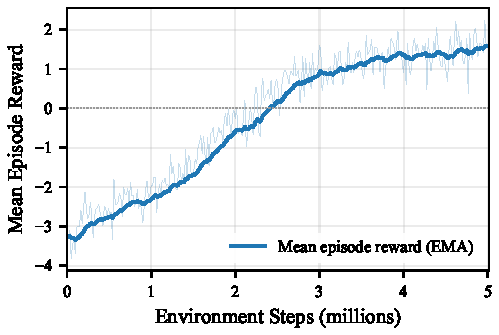
\includegraphics[width=\columnwidth]{figures/training_curves.pdf}
\caption{Mean episode reward during landing task training over 5M environment steps. The smoothed curve (EMA, $\alpha = 0.08$) shows a clear learning signal: reward transitions from negative (dominated by per-step costs) to positive (dominated by terminal landing bonuses) around 2M steps, indicating that the policy has learned controlled descent and soft touchdown.}
\label{fig:training_curves}
\end{figure}

The transition from negative to positive mean reward is significant: negative reward indicates that integrated per-step costs (attitude error, control effort, delta-v) dominate the return, while positive reward indicates that terminal landing bonuses ($+250$ success $+$ up to $+200$ pad accuracy) outweigh those costs. The crossover at $\approx 2$M steps marks the point where the majority of episodes end in successful landings rather than timeouts or crashes.


\section{Discussion}

\subsection{Effectiveness of Initialization Priors}

The throttle bias initialization proved essential for training stability. Early experiments without this bias (default throttle mean $\approx 0.5$) resulted in policies that immediately entered free-fall, accumulated large negative per-step rewards, and converged to a zero-throttle equilibrium---a local optimum where the agent minimizes per-step costs by crashing quickly. The initialization prior at 0.78 (near hover) ensures that initial rollouts produce meaningful flight trajectories from which the policy can learn descent behavior.

Similarly, the per-channel exploration noise initialization (quieter fins, louder throttle) addressed a failure mode where uniform exploration noise caused excessive lateral oscillations that prevented the policy from learning stable descent. With $\log\sigma_{\text{fin}} = -2.0$, the initial fin exploration is bounded to approximately $\pm 0.05 \cdot 0.262 \approx \pm 0.013$\,rad, small enough to avoid destabilizing the vehicle while still allowing gradient-based learning of fin control.

\subsection{Lateral Accuracy Challenge}

The primary open challenge is lateral accuracy: the policy reliably descends and lands softly but does not consistently steer toward the pad center. Several factors contribute to this limitation:

\begin{enumerate}
    \item \textbf{Throttle--fin coupling.} Lateral control authority depends quadratically on throttle. During descent, the policy reduces throttle below hover levels, which simultaneously reduces fin effectiveness. This creates a fundamental tension between descent rate and lateral controllability.
    \item \textbf{Actuator bandwidth.} The MG996R servos ($\tau = \SI{0.05}{\second}$, $\dot{\alpha}_{\max} = \SI{7.54}{\radian\per\second}$) limit the rate at which the policy can correct lateral errors, particularly during the final approach where corrections must be rapid.
    \item \textbf{Reward gradient at large distances.} The exponential pad accuracy bonus $e^{-d_{\text{horiz}}}$ has negligible gradient for $d > 2$\,m, where most of the descent occurs. While the linear horizontal position error term provides a constant gradient, its weight ($-0.30$) may be insufficient relative to the vertical speed shaping and delta-v cost terms that encourage rapid descent.
    \item \textbf{Spawn curriculum interaction.} The curriculum narrows the initial spawn range, which helps the policy learn on-pad behavior but may not provide sufficient training signal for large lateral corrections from the full $\pm 2.0$\,m range.
\end{enumerate}

\subsection{Comparison with Quadrotor RL}

Compared to quadrotor RL approaches \cite{b2, b3}, the TVC control problem presents unique challenges. Quadrotors have independent, throttle-decoupled attitude authority through differential rotor speeds, whereas the TVC vehicle's attitude control is fundamentally coupled to the thrust state. This coupling means that standard RL techniques developed for quadrotors---such as separate attitude and position control loops---do not directly transfer.

However, the single-actuator-plus-fins architecture also offers advantages: the 5-dimensional action space is smaller than a quadrotor's (typically 4 rotor speeds), and the vehicle's inherent aerodynamic stability (drag damping, gyroscopic stiffness) provides a degree of passive stabilization that aids learning.

\subsection{Sim-to-Real Considerations}

The simulation employs semi-empirical models calibrated to datasheet specifications and physical measurements. Key sources of sim-to-real gap include:

\begin{itemize}
    \item \textbf{Aerodynamic model fidelity.} The flat-plate fin model with empirical corrections may not capture flow separation, wake interactions between fins, or ground-effect changes during landing.
    \item \textbf{Servo nonlinearities.} Real MG996R servos exhibit backlash, load-dependent speed variation, and temperature drift not captured by the first-order model.
    \item \textbf{Battery voltage sag.} The 6S LiPo battery voltage drops under load, reducing available thrust during high-throttle maneuvers---an effect not modeled in the current simulation.
    \item \textbf{Sensor noise.} The simulation provides clean state observations, whereas the physical testbed will rely on noisy IMU and position estimates.
\end{itemize}

Domain randomization of these parameters during training is a natural next step for improving transfer robustness.


\section{Conclusion and Future Work}

This paper presented a PPO-based approach to controlling a thrust-vectored EDF VTOL vehicle in simulation. We developed a GPU-accelerated environment in NVIDIA Isaac Sim with semi-empirical propulsion, aerodynamic, and actuator models calibrated to a physical 3.1\,kg drone testbed. The key findings are:

\begin{enumerate}
    \item PPO can learn hover stabilization for a TVC vehicle, achieving \SI{0.085}{\metre} mean position error with a residual-PID architecture in only 2{,}048 environment steps.
    \item Pure PPO can learn autonomous landing with 100\% success rate and soft touchdowns (mean \SI{0.126}{\metre\per\second}), though lateral accuracy (mean pad distance \SI{1.89}{\metre}) remains an open challenge.
    \item Initialization priors on the action distribution (throttle bias near hover, per-channel exploration noise) are critical for avoiding degenerate local optima in TVC control.
    \item Terminal reward magnitudes must substantially exceed integrated per-step costs to prevent PPO from converging to cost-minimizing rather than task-completing policies.
\end{enumerate}

Future work will address the following directions:

\begin{itemize}
    \item \textbf{Gated Transformer-XL (GTrXL) policy.} Replacing the feed-forward MLP with a GTrXL architecture \cite{b16, b17} to provide temporal context for handling wind disturbances and improving trajectory planning during descent. Recent aerospace results \cite{b19, b20} suggest that transformer-based policies can improve landing performance under uncertainty, and the 24-dimensional observation space used here is compatible with the sequence-based input expected by GTrXL.
    \item \textbf{Domain randomization.} Randomizing aerodynamic coefficients, servo parameters, mass properties, and sensor noise during training to improve sim-to-real transfer robustness.
    \item \textbf{Lateral guidance improvements.} Investigating potential-based reward shaping (Ng et al., 1999), hierarchical policies (separate lateral and vertical controllers), and extended curriculum strategies to improve on-pad landing accuracy.
    \item \textbf{Hardware validation.} Deploying trained policies on the physical EDF drone testbed to validate sim-to-real transfer and characterize the reality gap.
    \item \textbf{Wind disturbance rejection.} Training and evaluating policies under stochastic wind conditions using the simulation's wind model, with the 27-dimensional observation space that includes wind estimates.
\end{itemize}

\section*{Data and Code Availability}

The simulation environment, training scripts, configuration files, and evaluation logs supporting this work are publicly available at \url{https://github.com/Jacob19999/Transformer-rl-retro-propulsion}.

\section*{Acknowledgment}

AI-assisted tools (Claude Opus 4.6, Anthropic) were used for code generation, debugging, and language editing during the preparation of this manuscript. All research design, simulation architecture, reward formulation, experimental execution, data analysis, and interpretation of results were performed by the author.

\begin{thebibliography}{00}
\bibitem{b1} R.~Beard and T.~McLain, \textit{Small Unmanned Aircraft: Theory and Practice}. Princeton University Press, 2012.
\bibitem{b2} J.~Hwangbo, I.~Sa, R.~Siegwart, and M.~Hutter, ``Control of a quadrotor with reinforcement learning,'' \textit{IEEE Robotics and Automation Letters}, vol.~2, no.~4, pp.~2096--2103, 2017.
\bibitem{b3} W.~Koch, R.~Mancuso, R.~West, and A.~Bestavros, ``Reinforcement learning for UAV attitude control,'' \textit{ACM Trans. Cyber-Physical Systems}, vol.~3, no.~2, pp.~1--21, 2019.
\bibitem{b4} C.~Pi, W.~Ye, and S.~Cheng, ``Robust quadrotor control through reinforcement learning with disturbance compensation,'' \textit{Applied Sciences}, vol.~11, no.~7, p.~3257, 2021.
\bibitem{b5} T.~Gaudet, R.~Linares, and R.~Furfaro, ``Deep reinforcement learning for six degree-of-freedom planetary powered descent and landing,'' \textit{Advances in Space Research}, vol.~65, no.~7, pp.~1723--1741, 2020.
\bibitem{b6} N.~Rudin, D.~Hoeller, P.~Reist, and M.~Hutter, ``Learning to walk in minutes using massively parallel deep reinforcement learning,'' in \textit{Proc. CoRL}, 2022, pp.~91--100.
\bibitem{b7} V.~Makoviychuk \textit{et al.}, ``Isaac Gym: High performance GPU-based physics simulation for robot learning,'' in \textit{Proc. NeurIPS Datasets and Benchmarks}, 2021.
\bibitem{b8} G.~Sutton and O.~Biblarz, \textit{Rocket Propulsion Elements}, 9th~ed. Wiley, 2017.
\bibitem{b9} J.~Luo, L.~Zhao, and C.~Cao, ``Research on the thrust vector control via jet vane in rapid turning of vertical launch,'' \textit{Journal of Mechanical Science and Technology}, vol.~32, no.~4, pp.~1823--1831, 2018.
\bibitem{b10} B.~Stevens, F.~Lewis, and E.~Johnson, \textit{Aircraft Control and Simulation}, 3rd~ed. Wiley, 2015.
\bibitem{b11} J.~Tobin, R.~Fong, A.~Ray, J.~Schneider, W.~Zaremba, and P.~Abbeel, ``Domain randomization for transferring deep neural networks from simulation to the real world,'' in \textit{Proc. IROS}, 2017, pp.~23--30.
\bibitem{b12} S.~Yu, J.~Tan, C.~K.~Liu, and G.~Turk, ``Preparing for the unknown: Learning a universal policy with online system identification,'' in \textit{Proc. RSS}, 2017.
\bibitem{b13} F.~Sadeghi and S.~Levine, ``CAD2RL: Real single-image flight without a single real image,'' in \textit{Proc. RSS}, 2017.
\bibitem{b14} J.~Schulman, F.~Wolski, P.~Dhariwal, A.~Radford, and O.~Klimov, ``Proximal policy optimization algorithms,'' \textit{arXiv preprint arXiv:1707.06347}, 2017.
\bibitem{b15} J.~Schulman, P.~Moritz, S.~Levine, M.~Jordan, and P.~Abbeel, ``High-dimensional continuous control using generalized advantage estimation,'' in \textit{Proc. ICLR}, 2016.
\bibitem{b16} E.~Parisotto \textit{et al.}, ``Stabilizing transformers for reinforcement learning,'' in \textit{Proc. ICML}, 2020, pp.~7487--7498.
\bibitem{b17} Z.~Dai, Z.~Yang, Y.~Yang, J.~Carbonell, Q.~Le, and R.~Salakhutdinov, ``Transformer-XL: Attentive language models beyond a fixed-length context,'' in \textit{Proc. ACL}, 2019, pp.~2978--2988.
\bibitem{b18} Q.~Li, S.~Peng, and S.~Levine, ``A survey on transformers in reinforcement learning,'' \textit{arXiv preprint arXiv:2301.03044}, 2023.
\bibitem{b19} L.~Federici, A.~Zavoli, and R.~Furfaro, ``Meta-reinforcement learning with transformer for lunar landing,'' in \textit{Proc. AIAA SciTech}, AIAA Paper 2024-2061, 2024.
\bibitem{b20} J.~Carradori, M.~Sagliano, and E.~Mooij, ``Transformer-based robust feedback guidance for atmospheric powered landing,'' in \textit{Proc. AIAA SciTech}, AIAA Paper 2025-2771, 2025.
\bibitem{b21} B.~A\c{c}{\i}kme\c{s}e and S.~R.~Ploen, ``Convex programming approach to powered descent guidance for Mars landing,'' \textit{Journal of Guidance, Control, and Dynamics}, vol.~30, no.~5, pp.~1353--1366, 2007.
\end{thebibliography}

\end{document}
